%%%%%%%%%%%%%%%%%%%%%%%%%%%%%%%%%%%%
\chapter{Algorithm}
\label{chap:Algorithm}
%%%%%%%%%%%%%%%%%%%%%%%%%%%%%%%%%%%%

This section provides detailed information on algorithm and its implementation.

\section*{Contribution Statement}

% STDMA协议的实现由supervisor提供,除此以外的所有其他部分均由本文作者独立完成
The implementation of the STDMA protocol is provided by the supervisor\footnote{\url{https://github.com/arthurrichards77/stdma_ros}}. Apart from this, all other components were independently completed by the author of this paper\footnote{\url{https://github.com/Vehshanaan/Dissertation2022}}.

\section*{Environment}
\label{chap:environment}
\begin{itemize}
    \item \textbf{Hardware:} ROG Zephyrus M16 Laptop
    \begin{itemize}
        \item CPU: 11th Gen Intel Core 17-11800H @ 2.30GHz
        \item GPU: NVIDIA GeForce RTX 3060 Laptop GPU (unrelated to the experiment, information provided just for content completeness)
    \end{itemize}
    \item \textbf{Software:}
    \begin{itemize}
        \item OS: WSL2 (Ubuntu 22.04 LTS) in Windows 11 23H2
        \item Implementation Platform: ROS2 Humble, all codes written in python
    \end{itemize}
\end{itemize}

\section{Communication with STDMA}

% 这是算法的第一部分:agent间的自组织通讯
This is the \textbf{first part of the algorithm: self-organised communication between agents}.

In STDMA, agents share a single channel by autonomously determining the serial speaking order, and the channel is represented with repeating frame with a certain number of discrete time slots.
The approach to determining the speaking order involves agents independently assigning the right to use available time slots within the channel.

\subsection{Synchronized Clock}

STDMA requires agents to have synchronized clock.

% STDMA假设agent之间拥有同步时钟。
\begin{quotation}
    \textbf{Assumption \arabic{Assumption}}: \stepcounter{Assumption} 
    Agents have synchronized clock. 
\end{quotation}

% 在实际中,同步时钟一般用GPS实现。在本文的模拟中,用一个ROS2publisher和一个topic来实现。
In practice, the synchronized clock is typically implemented with GPS. 
In the implemented simulation of this paper, it's \textbf{achieved using a ROS2 publisher and a topic}.
% 一个专用的ros2节点定时翻转其成员bool值,并在每次翻转此值时将翻转后的bool值publish到时钟topic中,这样在时钟topic中来形成一个占空比为50%的方波时钟信号。
A dedicated ROS2 node periodically toggles its member boolean value and publishes this boolean value to the clock topic each time it's toggled. This \textbf{creates a square wave clock signal with a 50\% duty cycle} in the clock topic.
% 其他普通agent通过订阅时钟话题的方式来获得同步时钟信号。
Agents obtain the synchronized clock signal by subscribing to the clock topic.

% 信道时间的离散化
\subsection{Discretization of Channel Time}
\label{chap:sending time window}
% agent将一个完整的时钟信号周期视作一个slot,将若干slot视作一帧。
Agents consider a complete clock signal period (a high and a low) as one slot and consider a specific number of slots as a frame.
Time frames continuously cycle, providing continuous and reusable slot resource for agents to use.


\begin{quotation}
    \textbf{Assumption \arabic{Assumption}:} \stepcounter{Assumption} 
    The number of slots in a frame is predefined within the agents, and this parameter value is the same for all agents.
\end{quotation}

% 注意,不要求各agent的帧起始点相同,允许agent有不同的agent起始点offset

Please note that it is not necessary for each agent to have the same starting point for their frame. 
In other words, agents are permitted to have different frame starting point offsets.

% agent在槽的正中央发送消息。
The exact middle of each slot is the timing for message transmission.
This divides a slot into two parts: before sending the message and after sending the message.

\begin{figure}[htbp]
    \centering
    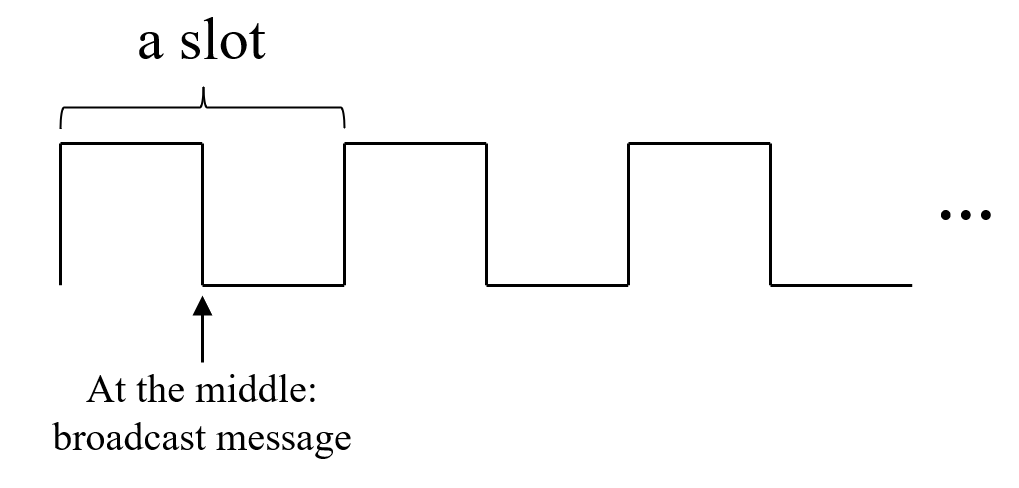
\includegraphics[width = 0.6\linewidth]{figures/slot_discretisation.png}
    \caption{Illustration of the clock signal, slot structure, and the timing for message broadcasting within a slot.}
    \label{fig:slot_discretization}
\end{figure}
\FloatBarrier

\subsection{State Machine for Channel Allocation}
\label{chap:stdma statemachine}

% 使用STDMA的agent有四个阶段,每个阶段对应一个在网络中的状态。因此,agent加入网络的过程可以用状态机来管理,随着状态逐步转化,agent逐步加入网络并获得自己的槽
Agents employing STDMA go through four phases\cite{STDMA}, with each phase representing a stage in an agent's integration into the network. Consequently, a state machine can effectively manage the process of an agent joining the network. Through progressive state transitions, the agent incrementally integrates into the network and secures its slot.



% 本文中对此状态机的实现如下:
The implementation of this state machine in this paper is as follows:


\begin{figure}[htbp]
    \centering
    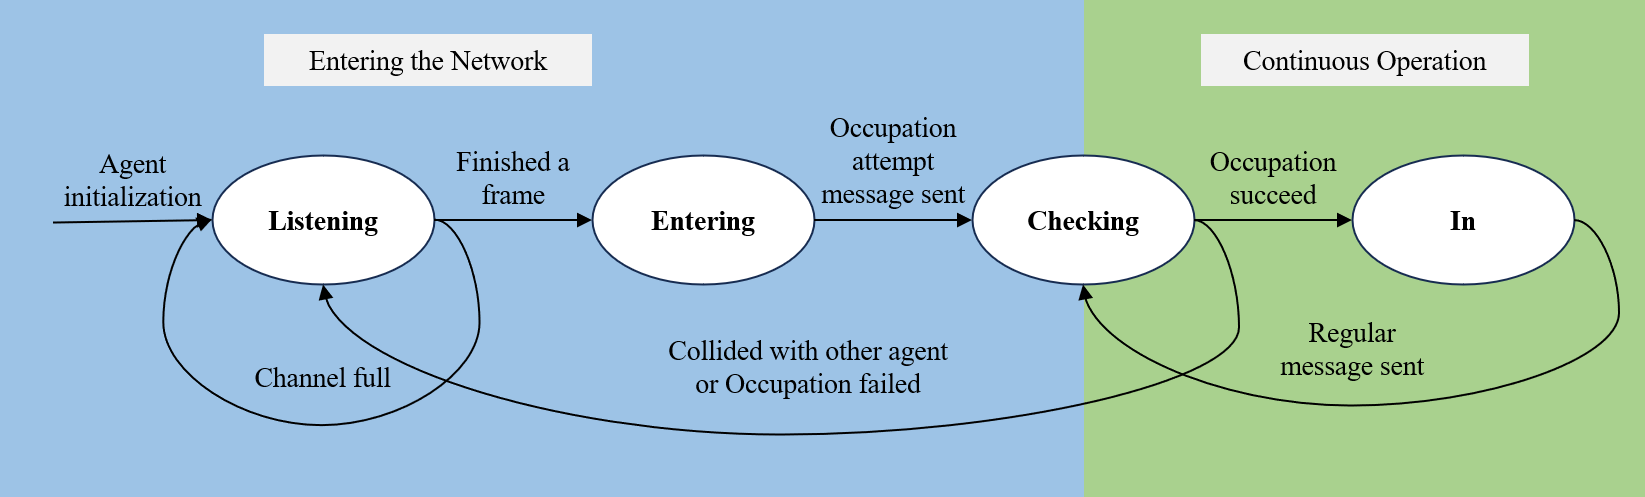
\includegraphics[width = \linewidth]{figures/state_machine.png}
    \label{fig:state machine}
    \caption{Schematic diagram illustrating the agent's state machine for managing STDMA.} 
\end{figure}

\begin{enumerate}
    \item \textbf{Listening}
    
    % 在此状态下的agent如何如何如何

    % 此状态下的agent的目的是确定当前的信道槽位分配情况,此状态下的agent尚未进入网络
    In this state, the agent's objective is to determine the current channel slot allocation by 'Listening' to the channel. 
    Agents in this state have not yet joined the network.

        \textbf{Slot allocation determination}: 
        
        In a slot:
    \begin{itemize}
        % 如果仅收到一条消息:槽有主
        \item If only one message was sent: the slot is occupied by the sender.
        % 如果收到多条消息
        \item If multiple messages were sent or no message was sent: the slot is considered free.
    \end{itemize}

    The initial state of an agent is this state.

    % Transition Condition: 每次听完完整的一帧后,agent尝试离开此状态
    \textbf{Transition Condition}: After listening to a complete frame, the agent attempts to exit this state.
    \begin{itemize}
        % 当信道中有一个或多个未被使用的槽时,进入entering状态
        \item $\rightarrow$ Entering: There are one or more unoccupied slots within the frame.
        % 信道中无空闲槽时:呆在listening.
        \item $\circlearrowleft$ Listening: There are no free slots remaining in the frame. This suggests that the channel's capacity has been fully utilized, and the agent can only stay 'Listening' and remain idle.
    \end{itemize}
    
    \item \textbf{Entering}
    
    % 在此状态下的agent的目的是如何,agent的状态是如何
    In this state, the agent attempts to occupy a free slot in order to try 'Entering' the network.

    % Transition Condition: 
    \textbf{Transition Condition}: 
    % Agent尝试占用一个随机的在lisening状态中确认的free slot.
    Agent randomly selects one from the free slots determined while in the 'Listening' state.
    % 在这一槽中,agent发送其id,来尝试获得此槽
    Within this slot, the agent \textbf{transmits its unique ID} in an effort to occupy the slot.

    \begin{itemize}
        \item $\rightarrow$ Checking: The agent transitions to the 'Checking' state immediately after sending the occupation attempt message.
    \end{itemize}


    \item \textbf{Checking}
    
    % 在此状态下的agent的目的是如何,agent的状态是如何
    % 此状态下的Agent刚刚在某一槽中发布了一条信息,需要根据槽内收到的消息的数量判断自己对此槽的所有权。
    In this state, the agent has just broadcasted a message in a specific slot and must ascertain its ownership of that slot with the quantity and content of messages received within that slot.
    % 通过检查自己对此槽的所有权,变更自身状态。
    By 'Checking' its ownership of that slot, the agent transits its state.

    % 注意,未进入网络和已进入网络的agent都会在发布消息后进入此状态。
    Note that both agents that have not yet entered the network and those that have will transition to this state after sending a message.

    % Transition Condition:
    \textbf{Transition Condition}: Transition the state based on the quantity and content of messages received in the slot where a message has been sent.
    \begin{itemize}

        % 如果只收到一条消息且来自自己:说明自己拥有此槽位,即在网络中
        \item $\rightarrow$ In: If only one message is received, and it's from itself (received ID = self ID), it indicates that the agent has ownership of that slot, meaning it is 'In' the network.
        % 任何其他情况:自己不拥有此槽位,重新尝试获得槽位。
        \item $\rightarrow$ Listening: In \textit{any other situation}: The agent does not have ownership of that slot and should try to secure a slot again.
        
        % 解释:所有其他情况包含:
        \textbf{Explanation: All other situations include}:
        \begin{itemize}
            % 没有收到自己的消息
            \item Didn't receive its own message: This suggests that either the broadcast was unsuccessful or the reception was unsuccessful (e.g., due to hardware damage or scheduled broadcasting being prevented, etc.). In both situations, we do not want the agent to enter the network, as its communication function may not be consistently reliable.
            % 多个节点尝试在同一槽内发送消息:
            \item Multiple agents sent messages within one slot (i.e. collision):
            
            % 碰撞情景1:多个正在进入网络的agent恰好选择了同一个槽位。此种碰撞在本算法框架下无法避免,但由于仅发生在未进入网络的agent之间,对其他有效通讯没有影响。
            \subitem Collision Scenario 1: Multiple agents attempting to join the network coincidentally select the same slot. While such collisions are unavoidable within the context of this algorithm, they only occur among agents that have not yet entered the network and thus do not impact other normal communications.
            
            % 碰撞情景2:已加入网络的agent与未加入网络的agent发生碰撞。此种碰撞在理论上是不应该发生的,因为未加入网络的节点应当只尝试获得未被使用的槽位。若agent错过了时钟脉冲,则可能会出现此种情况。若某agent失去时钟脉冲,则会导致其和所有其他agent失去同步,进而导致事故。这一情况要尽可能避免。
            \subitem Collision Scenario 2: A collision occurs between an agent that has already joined the network and one that has not. In theory, this type of collision should not occur, as agents not yet in the network should only attempt to occupy unoccupied slots. However, this situation may arise if an agent misses a clock pulse. Missing a clock pulse can cause an agent to fall out of synchronization with all other agents, potentially leading to conflicts and accidents. Efforts should be made to prevent this situation as much as possible.
        \end{itemize}

    \end{itemize}    


    \item \textbf{In}
    
    % 在此状态下的agent的目的是如何,agent的状态是如何
    % 在此状态下的agent已经进入网络,且应当始终在网络中,直到其通过停止定期发送消息来放弃其槽位。
    In this state, the agent is 'In' the network and should stay in the network until it releases its slot by stopping its regular message transmission.
    
    % agent在抵达终点后,将会关机并放弃自己在信道中的槽。
    Upon reaching their destinations, agents will shut down and release the slot they occupied in the channel.
    
    \textbf{Shut Down and Release Slot}:
    % agent只要停止在自己已有的槽中发送消息就可以放弃对这个槽的使用权。
    An agent can release its allocated slot simply by ceasing to send messages within that slot.
    
    % Transition Condition:
    \textbf{Transition Condition}:
    \begin{itemize}
        % 每次发送消息后,检查自己对此槽的所有权
        \item $\rightarrow$ Checking: After publishing a message, verify ownership of that slot.
    \end{itemize}

\end{enumerate}


\comment{
\subsection{Summary}

% 实现了agent的自组织无碰撞信道分享。信道的时间被表示为包含指定数量槽的重复的帧,
% agent通过尝试占有帧中一个槽的方式来加入网络,此过程由状态机管理并实现。
This achieves agent self-organization and collision-free channel sharing. The channel's time is represented as repeating frames containing a specified number of slots. An agent attempts to join the network by trying to occupy one slot within a frame, the joining process is managed and implemented by a state machine.
}


\section{Path Planning and Sharing}

This is the \textbf{second part of the algorithm: collision-free movement planning for multiple agents}.


% agent的移动模型, 计划的作用,分享的方式
\subsection{Basic Framework and Definitions}


\subsubsection{Map}
The map is a grid world with obstacles, and the map information is pre-loaded into the agents:
% 本文中所使用的地图仅包含静止障碍物
\begin{quotation}
    \textbf{Assumption \arabic{Assumption}}: \stepcounter{Assumption}
    % 所有的障碍物都是静止的
    All obstacles in the map are stationary, and map information is pre-loaded into agents.
\end{quotation}

\subsubsection{Agent Capabilities and Constraints}


\begin{quotation}
    \textbf{Assumption \arabic{Assumption}}: \stepcounter{Assumption}
    % agent的capabilities是相同的。
    Agents are identical.
\end{quotation}

\textbf{Capabilities}:
\begin{itemize}
    % 每时间步可以不动或移动一格
    \item Moving: Agents can choose to either remain stationary or move to an adjacent non-diagonal grid cell at each time step (corresponding to a time slot in the STDMA channel).
    % 可以完美执行计划
    \item Model Predicting: Agents can execute their own plans with complete accuracy.
\end{itemize}

\begin{quotation}
    \textbf{Assumption \arabic{Assumption}}: \stepcounter{Assumption} 
    % agent的移动不受外部扰动的干扰,且对自己运动的预测百分之百准确。
    The agent's movement is not affected by external disturbances, and its prediction of its own motion is completely accurate.
\end{quotation}

Note: \textbf{Agents do not have perception of their surroundings}, and they achieve collision-free movement solely based on predictions of other agents' moves.



\textbf{Constraints}

\begin{itemize}
    % 不能碰撞
    \item No Collision: Agents should not collide with each other.
    % 不能穿墙
    \item Obstacle Avoidance: Agents should not use positions on the map that are occupied by obstacles.
\end{itemize}

\subsubsection{Collision Definition}

% 在本文中,以下两种情形被视为碰撞:
In this paper, the following two scenarios are considered as collisions:
\begin{itemize}
    % 两个或以上节点在同一时刻位于地图上的同一2D位置
    \item Two or more agents are located at the same 2D position on the map at the same time (Fig \ref{fig:Collision1}).
    % 两个节点交换位置。即,t时刻agentA位于位置a,agentB位于位置b,t+1时刻A位于b,而B位于A
    \item Two agents swapping their positions. That is, at time $t$, agent $A$ is at position $a$, and agent $B$ is at position $b$. At time $t+1$, agent $A$ is at position $b$, while $B$ is at position $a$ (Fig \ref{fig:Collision2}).
\end{itemize}

\begin{figure}[htbp]
    \centering
    \begin{subfigure}[t]{0.6\linewidth}
      \centering
      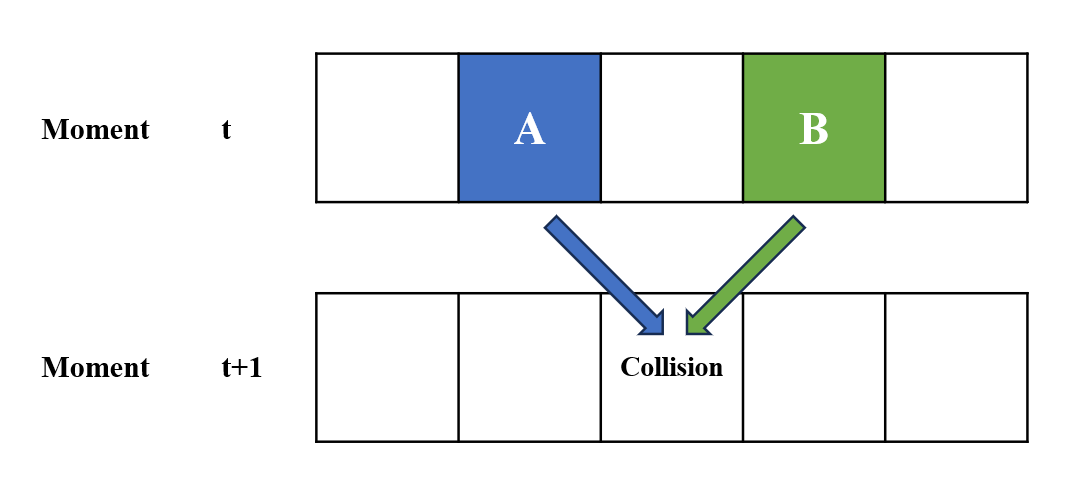
\includegraphics[width = \linewidth]{figures/Collision1.png}
      \caption{Collision Scenario 1: Two agents attempting to occupy the same position simultaneously.}
      \label{fig:Collision1}
    \end{subfigure}
    \begin{subfigure}[t]{0.6\linewidth}
        \centering
        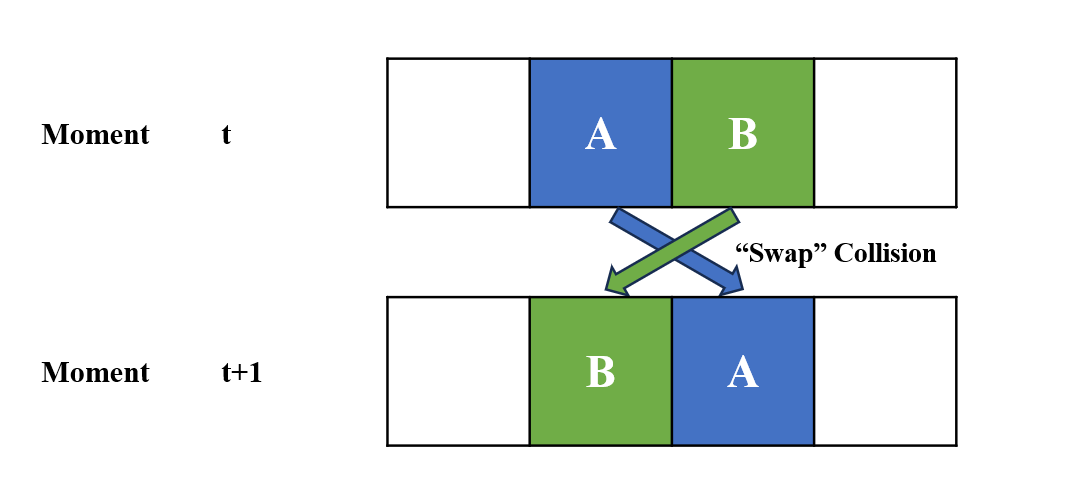
\includegraphics[width = \linewidth]{figures/Collision2.png}
        \caption{Collision Scenario 2: Two agents swap their positions.}
        \label{fig:Collision2}
      \end{subfigure}
    \caption{Illustration of collision scenarios.}
    \label{fig:Collisions}
\end{figure}

\subsubsection{Plan Definition and Constraints}

\textbf{Definition}

% 计划的定义就是一串三维坐标点,其中每个坐标点都由一个二维坐标和一个时间点构成。
A plan is a sequence of 3D coordinate points $(x,y,t)$. Each coordinate point comprises a 2D location $(x,y)$ and a specific time $t$, essentially indicating both the spatial and temporal aspects.
% 由于agent mobility的约束,计划中相邻点的二维坐标部分必须为非对角的相邻点。此外,计划中的相邻点的时间点也必须是单调以1的步长递增。


% 计划的约束
\textbf{Constraints}

% 计划的约束是:1. 不能与其他agent或地图中的障碍物发生碰撞。 2. 计划中相邻的点,空间上必须是非对角的相邻点,时间上后一点必须比前一点增加1。 3. 计划的第一个点必须在空间上与开始计划时刻的agent位置位于非对角的相邻点。
\begin{enumerate}
    % 计划中的点必须符合agent的移动能力与约束
    \item The points in the plan should align with the agents' capabilities and constraints (collision-free, move no more than one grid at a time).
    % 计划中的第一个点必须是是agent开始计划时刻的位置的非对角相邻点,且满足agent的其他约束
    \item The first point in the plan should be a non-diagonal adjacent point to the agent's initial position at the start of planning, and it must also satisfy the agent's other constraints.
\end{enumerate}



\subsection{Plan Broadcasting Method and Time Window for Planning}

\subsubsection{Broadcasting}

% agent通过stdma所分享的信道进行自身计划的分享,即,在每个属于自己的槽的中央在信道中广播自身的计划。
Through the channel facilitated by STDMA, agents broadcast their individual plans. 
This means \textbf{agents broadcasting their new plans and their IDs in the middle of each slot allocated to them} within the channel (see Fig \ref{fig:slot_discretization} in Section \ref{chap:sending time window}).

% 注意,计划制订时仅生成二维坐标的序列,时间在计划过程中是隐含的。计划中的时间维度在计划被接收时由接收者自己添加。
Note that during plan formulation, only a sequence of 2D coordinates is generated, and time is implicit in the planning process. The time dimension of the plan is added by the recipient upon receiving the plan.
% 因此,每次仅传输一组二维坐标序列即可。
As a result, only a set of 2D coordinate sequences needs to be transmitted each time broadcasting.

% 此外,还有一个称为plan length limit的参数,每次广播时所广播的计划长度不可超过此长度。
Additionally, there is a global parameter called "\textbf{\textit{plan length limit}}", the length of the plan broadcasted each time window should not exceed this limit. 
The portion of the plan that exceeds this length will be truncated and abandoned.

\begin{quotation}
    \textbf{Assumption \arabic{Assumption}:} \stepcounter{Assumption} 
    The plan length limit is predefined within the agents, and this parameter value is the same for all agents.
\end{quotation}

% 计划的时机
\subsubsection{Time Window for Planning}
\label{chap:time window for planning}

% 如前文所述,每个agent在属于自己的槽的中间发布信息。
As previously mentioned in Section \ref{chap:sending time window}, each agent publishes their message in the middle of the slot allocated to it.
% 基于这一特性,对于每个agent来说,存在这样一个定期出现的时间窗口:涉及计划制订的所有变量都是确定的,且自己的计划只要制订完成就可以立即发布。
Based on this rule, for every agent, \textbf{there exists a periodically repeating time window where all variables (map, others' plans) related to planning are constant}, 
and the agent's own \textbf{plan can be immediately published as soon as it is formulated}.

% 这个时间窗口就是自己的槽的前半部分。在这段时间内,不会有其他agent发布新的计划,且此时段结束后就可以立即发布自身的计划。
This time window is the first half of the agent's own slot. Within this interval, no other agents would broadcast new plans, and as soon as this interval ends, the agent can immediately publish its own plan.
% 由于此窗口是一个槽,这一窗口在每一帧中会出现一次
This time window is \textbf{guaranteed to occur once in each frame} because it is a segment of a certain slot. 

\begin{figure}[htbp]
    \centering
    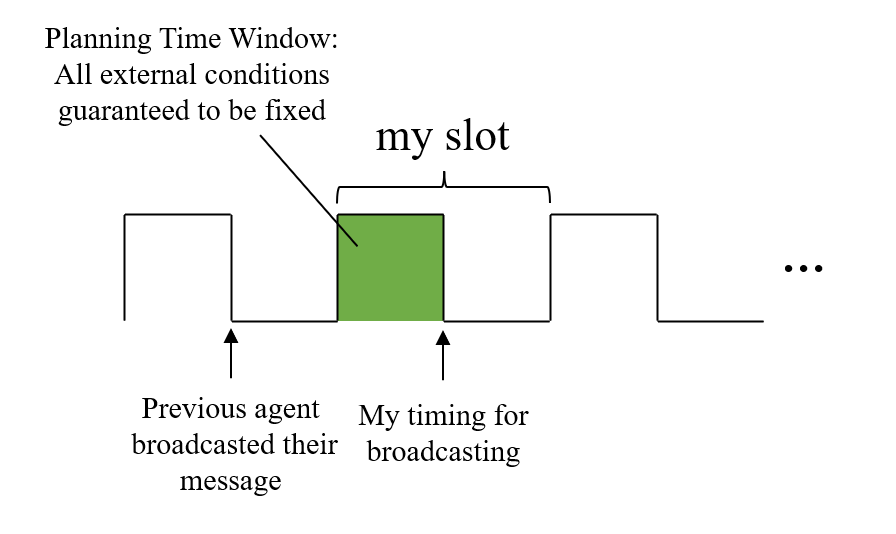
\includegraphics[width = 0.7\linewidth]{figures/PlanningTimeWindow.png}
    \label{fig:PlanningTimeWindow}
    \caption{Illustration of planning time window.}
\end{figure}

\subsection{Plan Generation}
\label{chap:plan generation}

% 每次计划时,agent遍历planning horizon以内的所有满足约束的可能计划(即路径),并选择能令agent最大化接近终点的计划.
Each time planning, agent traverses all potential plans (i.e., paths) within the global parameter \textbf{\textit{planning horizon}} that satisfy the constraints (moving capabilities and collision-free) and choose the plan that brings the agent closest (judged with Manhattan distance) to the goal.

\begin{quotation}
    \textbf{Assumption \arabic{Assumption}:} \stepcounter{Assumption} 
    The planning horizon is predefined within the agents, and this parameter value is the same for all agents.
\end{quotation}

% 由于agent的计算能力限制,只能在每个planning time window中遍历固定距离的未来。这一值是根据agent的计算能力确定。
\textbf{Explanation on planning horizon}: Due to the computational limitations of the agent, it can only traverse a fixed distance into the future within each planning time window. This value is determined based on the agent's computational capacity.

\textbf{Method for traversing potential plans}: 
% agent用A*来遍历可能性空间,采用的启发式函数是位置与goal的曼哈顿距离。
The agent employs the \textbf{A* algorithm} to navigate the possibility space, adopting the Manhattan distance between the current position and the goal as the heuristic function.
% 注意,此处的可能性空间是由二维地图和时间构成的三维空间。
Note that in this context, \textbf{the possibility space is a 3D space} composed of the 2D map and time.


% 模型预测和receding horizon
\subsection{Model Prediction}
\label{chap:model prediction}

% agent通过Model Prediction来生成满足约束的计划。
Agents generate plans that meet the constraints through model prediction.

\subsubsection{Principles}

% Model Prediction 通过以下两条关于agent行动的共识实现:
Model Prediction is implemented based on two agreed-upon principles concerning agent behaviour:
\begin{itemize}
    % 1. agent会准确执行自己发布过的计划
    \item Principle 1: Agents would accurately execute all published plans.
    % 2. 若某agent在两次计划窗口间用尽了自身的计划,则此agent在这一帧剩余的时间中保持静止
    \item Principle 2: If a particular agent exhausts its own plan between two planning windows, it remains stationary \textbf{for the remainder of that frame}.
\end{itemize}

\subsubsection{The Purpose of Principle 2 and the issues it generates:}

\textbf{Purpose}: Decouple the frame length and the computational ability of agents. 

    % 共识2可使agent在无计划可用时也有可采取的行动,且不会从其他agent的感知中消失(因为agent只靠计划相互感知)。若没有共识2,则每次计划时必须能够生成长度大于等于帧长度的计划,这是一种对帧长度的不必要的限制。
    Principle 2 ensures that agents always have an available default action and remain perceptible when their plans are exhausted (since agents percept each other solely through prediction). Without Principle 2, agents must generate a plan equal or longer than frame length, which imposes an unnecessary constraint on the frame length.

\textbf{Problem}: 
    % 由于待在原地并不是通过计划生成的安全行为,这有可能会导致潜在的与其他gent的计划的碰撞。
    Given that remaining stationary is not a safety behaviour generated through planning, it can potentially result in collisions with the plans of other agents.
    % 为此,只要使agent保持静止的时域内没有其他agent的计划就可以了。
    \textbf{To prevent collisions, we must make sure no other agents have plans at in the time domain which one agent decides to remain stationary.}
    % 全局变量 planning horizon和plan length limit保证了这一点。
    The global parameters \textit{\textbf{plan length limit}} and \textit{\textbf{planning horizon}} are in place to make sure of that. These two parameters guarantee that \textbf{all agents in the system broadcasts plans of the same length each time broadcasting}.
    
    % 当一个agent计划时,它的planning horizon前沿就是整个系统的predicting horizon前沿,此时必定没有其他agent的计划,而后续agent的计划会将之前agent采取的原地静止纳入考虑,从而保证了无碰撞。
    When an agent is planning, the leading edge of its planning horizon matches the leading edge of the entire system's predicting horizon (Fig \ref{fig:RecedingHorizon}). And no plan from any other agent could reach this far. Plans made by agents afterward will take into account the stationary position adopted by the earlier agents, ensuring no collisions


\begin{figure}[htbp]
    \centering
    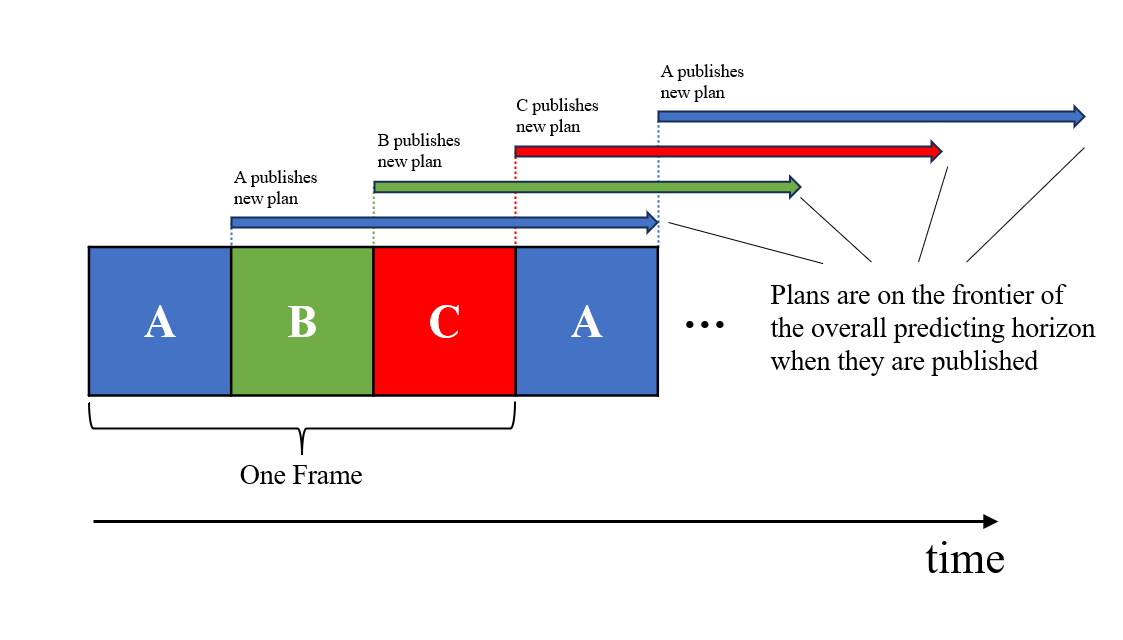
\includegraphics[width = \linewidth]{figures/RecedingHorizon.png}
    \caption{Illustration of 3 agents within a channel having a frame length of 3, where agents publish plans of equal length. This demonstrates why new plans are always on the frontier of the overall predicting horizon.}
    \label{fig:RecedingHorizon}
\end{figure}

\comment{
% 本文中通过假设agent可以绝对准确执行自身计划的方式对模型预测进行了大幅度简化。
In this paper, the model predictions have been significantly simplified by assuming that agents can execute their own plans with absolute accuracy.

% 对agent的模型预测遵循以下两条规则:
Agents follow the rules below to predict their own and other agents' movements:
\begin{enumerate}
    % 发布的计划一定会得到执行。
    \item A plan that has been published will definitely be executed.
    \item If an agent exhausts its plan before its planning window arrives, the agent will execute a default behaviour: remaining stationary. This will continue until the agent publishes a new plan.
\end{enumerate}

% 默认行为将帧长度和计划长度解绑,因为即使agent无法生成足够一帧使用的计划,也可以通过执行默认行为来等待下一次计划窗口的到来。
The default behaviour decouples frame length from plan length. This is because, even if the agent cannot generate a plan sufficient for a whole frame, it can still execute the default behaviour, waiting for the next planning window to arrive.

% 上述的默认行为带来了一个问题,就是默认行为并不遵循无碰撞约束,agent在原地待机时可能会占用其他agent在未来使用的位置,从而产生碰撞。
And this default behaviour presents an issue: it doesn't adhere to the non-collision constraint. An agent, while idling in place, might occupy a position that another agent intends to use in the future, leading to collisions.
% 为了解决这一问题,将全体agent所能生成的计划的长度设定为一个统一值。
To address this concern, the length of the plans that all agents can publish is set to a uniform value.


% 这样,由于agent依次计划且计划长度统一,每次计划的结尾都将是系统总体horizon的最前端,从而可以在这里执行默认行为(原地待机)而不与其他计划发生冲突,因为在这个时间范围内没有其他计划。agent进行计划时,将其他agent结束计划后的原地待机纳入考虑,即可避免与待机agent发生碰撞。
In this way, since agents plan sequentially and with a uniform plan length, the end of each plan will always coincide with the leading edge of the system's overall horizon. This allows them to execute the default behaviour (idling in place) at this point without conflicting with other plans, since no other plans exist within this time frame. When an agent formulates its plan, it takes into consideration the idling of other agents after their plans have concluded, ensuring it avoids collisions with agents that are stationary.

\textbf{ADD PIC HERE} % 画图,展示为什么默认行为得位于尖尖上。

% 也是因为这个原因,每次寻路算法都冷启动,因为每次计划必须生成同样长度的计划,就必须用最坏情况来对计划长度进行限制。最坏情况是agent必须舍弃所有的先前工作,从头开始进行计划。由于这一原因,热启动寻路算法不能提高算法性能及planning horizon.
For this reason, the pathfinding algorithm always starts from scratch. Since each plan must be of the same length, the plan length is constrained by the worst-case scenario. In the worst case, an agent must abandon all previous work and start planning anew. Due to this, a warm start for the pathfinding algorithm does not improve algorithm performance or the planning horizon.

% 注意,当发布的计划长度超过帧长度时,不继承上次计划结果和发布的计划一定会被执行是不矛盾的。以单个agent的前后两次计划为例,第一次计划并发布后,其他agent会在后续计划时基于这个已发布计划规划自己的路径,确保不使用第一次计划中的位置。第二次计划时,即使不直接继承第一次计划中未用完的部分,由于此时计划不可能比上次计划更优,求解的结果还是一样的。相当于隐式继承了已发布但未使用的部分计划。
Note, when the length of a published plan exceeds the frame length, it isn't contradictory to the idea that a plan once published will definitely be executed and not inheriting the results from the previous plan (cold start planning). Take the sequential plans of a single agent as an example: after the first plan is made and published, other agents, in their subsequent planning, will draft their paths based on this released plan to ensure they don't occupy positions specified in the first plan. During the second planning, even if it doesn't directly inherit the unused portions of the first plan, since the planning at this point can't possibly be better than the previous one, the resulting solution remains the same. This is akin to implicitly inheriting the parts of the plan that were published but not utilised.

% 在算法实现中,通过给计划长度加一个全局统一的上限(plan length limit),并根据agent计算能力为单次计算中可预测的未来的长度加一个上限(planning horizon)来实现此功能。
In the algorithm's implementation, this functionality is achieved by imposing a globally uniform cap on the plan length (referred to as the 'plan length limit') and setting an upper boundary for the foreseeable future that can be predicted during a single computation, known as the 'planning horizon', based on an agent's computational capacity.
}

\subsubsection{Cold Start of Planning}

% Cold start of planning是指每次计划时,agent都从自己当前的位置开始生成计划,不从先前的计算中继承任何数据。这样做是有原因的:
'Cold Start of Planning' refers to the initiation of the planning process by an agent from its current position, \textbf{without inheriting any data from previous computations}. There are justifiable reasons for adopting this approach:

% 如前所述,agent每次必须生成固定长度的计划。
As previously mentioned, \textbf{agents are required to generate and publish plans of a fixed length each time they plan.
% 这就意味着,这一固定长度受到最坏情况的制约。
% 在最坏情况下,前一agent新发布的计划使得当前agent的全部未发布计划作废,必须从头冷启动计划生成算法。
This fixed length is constrained by worst-case scenarios.} In such scenarios, a newly published plan from a preceding agent may invalidate all unpublished plans of the current planning agent, leading to a cold start in the planning algorithm.
% 必须保证即使在这一情况下agent仍能生成固定长度的计划。因此,即使不冷启动planning,计划长度的瓶颈也不会改变,因此每次都冷启动planning.
\textbf{It is crucial to ensure that even in these worst-case scenarios, the agent can still generate a plan of fixed length}. Therefore, the bottleneck of plan length remains unchanged whether a cold start is implemented in the planning process or not.

% 此外,若发布的计划长于一帧,冷启动不会导致agent在第二次计划中采取和前次计划不同的行动,因为不会有能使最优计划改变的条件出现。
Additionally, if the published plan spans more than a single frame, a portion of the plan would be in a state of having been published but not yet executed. \textbf{Even with a cold start, the newly generated plan will still include this unexecuted portion of previous plan}, as no new variables could alter this solution (cannot have better solution: plan from other agents could only increase; cannot have worse solution: other agents avoid positions in published plans, and obstacles in the map are stationary).


% agent进入地图的流程
\subsubsection{The process of an agent entering and exiting the map}
\label{chap:behaviour}
\label{chap:join map}

\textbf{Entering the map}: 

% 由于agent之间的感知只依靠计划和对默认行为的共识,agent在进入网络并成功生成计划前是不为其他agent所知的,这可能导向潜在的碰撞。因此,agent在开机时并不在地图中占据位置,而是遵循以下流程来进入地图:
Since agents' awareness of each other relies solely on planning and consensus on default behaviour, \textbf{an agent is not known to others before it enters the network and successfully publishes a plan}, which can lead to potential collisions. Therefore, when an agent starts up, it does not occupy a position on the map; instead, it follows the following process to enter the map:

\begin{itemize}
    % agent尝试加入网络
    \item The agent attempts to join the network.
    \item The agent tries to generate a plan with its starting point as the origin. If successful, it executes according to the plan (thus acquiring a place on the map). If unsuccessful, it repeatedly attempts to generate this plan.
    \item The agent operates continuously on the map.
\end{itemize}

% 由于后续实验中将起点设置为位于地图边缘,这一过程可以视为agent尝试进入某一区域的网络并进入某一区域的过程。
Due to the subsequent experiments setting the starting points at the edge of the map, this process can be regarded as the agent's attempt to enter a specific area's network and subsequently its entry into that area.

\textbf{Exiting the map}:
\label{chap:exit map}

% agent只要发现自己抵达终点,就退出地图:不再在地图中拥有位置,且放弃自己在信道中的槽(停止向stdma信道中发送信息即可)。
Once an agent detects its arrival at the goal, it exits the map: it no longer holds a position within the map and relinquishes its slot in the channel (by ceasing to transmit information to the STDMA channel).

Due to the subsequent experiments setting the goals at the edge of the map, this process can be regarded as the agent exiting a specific area's network and leaving that area.


\subsection{Path Planning Function and Implementation}

% 在每个计划窗口开始时,计划函数被调用,用以生成接下来agent的移动计划。
At the start of each planning window, the path planning function is called to generate the upcoming movement plan for the agent.

\subsubsection{Inputs of the function}

\begin{enumerate}
    % 地图,自己的当前位置,目标点,其他agent的计划
    \item \textbf{map, agent's current position, goal, plans of other agents}

    % 这些是计划所需的基础信息。
    Foundational information required for the planning process.

    % 是否是第一次进入地图? 
    \item \textbf{first ever plan}
    
    % 这是一个bool值,指示当前计划是否为agent的进入地图时的首个计划,其初始值为False.
    This is a boolean value that indicates whether the current plan is the agent's first plan upon entering the map, with an initial value of False.


    % 这是为了前述的agent进入地图的流程而准备的参数。此值为真时,计划的首个点必须为agent的起点。此值为假时,计划的第一个点从agent当前位置的相邻点中选出
    This parameter is prepared for the aforementioned (Section \ref{chap:join map}) process of an agent entering the map. When this value is true, the first point of the plan must be the agent's starting point. When this value is false, the first point of the plan is selected from points adjacent to the agent's current position.
    % 当agent成功生成首个计划后,此bool值则翻为真。
    Once the agent successfully generates its first plan, this boolean value is set to True.


    % horizon
    \item \textbf{planning horizon}

    Previously mentioned in Section \ref{chap:plan generation}.

    % 在单次计划中所探索的时间范围上限。若一个可能计划的长度达到此值,则该计划将不再被扩展,转而扩展其他未达到此长度的计划
    The upper limit of the time range explored within a single plan session. 
    If a possible plan reaches this length, it will no longer be extended, and other potential plans that have not reached this length will be extended instead.
    % 若horizon内的所有可能性被探索完或产生了抵达终点的计划,则停止计划,返回生成的计划中能令agent最大化接近终点的计划。
    If all possibilities within the horizon have been explored or a plan that reaches the goal has been generated, planning is stopped, 
    and the plan that allows the agent to approach the goal most closely among the generated potential plans is returned.



    % 所需计划之长度
    \item \textbf{plan length limit}
    
    Previously mentioned in Section \ref{chap:time window for planning}
    
    % 这一参数的目的是限制返回的计划的长度上限。仅返回生成的计划中不超过此长度的部分。
    The purpose of this parameter is to limit the maximum length of the returned plan. Only the portions of the generated plan that do not exceed this length are returned (and then published).
    

    
    % 每次生成计划时要求生成的
\end{enumerate}

% 创建一个成员为当前位置的openset(即已发现但还未访问的点)。起点的时间维度为0(对应正在计划的这一槽)
% 当openset不为空时:
%   从openset中弹出综合代价 = 耗时+启发式代价(距终点曼哈顿距离)最低的点及其所对应的路径。
%   如果路径长度大于等于horizon:continue
%   如果此点是终点且耗时<=required length: 返回路径。
%   获得此点的可用邻居点(位于地图中可用点且不与其他agent发生碰撞,且不位于closedset的点)作为待扩展点
%   邻居点的时间戳是当前点+1。
%   若是第一次计划,则可用邻居点(下一步待扩展点)必须为起点。
%   将待扩展点推入openset中。
%   将此点推入closedset中。
% 从closedset中选出对应路径离终点的综合代价最低的,返回此路径
% 若closedset为空且agent是第一次计划:返回空。此时地图中没有足够的供其进入的空间。

\begin{algorithm}[H]
    
    %\small
    %\SetNlSty{}{}{}{}{}{}
    %\SetNlSty{textbf}{}{}{}{}{}
    \setstretch{1.1}


    \caption{Path Planning Function}
    \label{alg:path_plan}
    \DontPrintSemicolon % 不要分号
    
    \SetKwFunction{pathplan}{path\_plan}
    \SetKwProg{Fn}{Function}{:}{}
    \SetKwIF{If}{Elseif}{Else}{if}{then}{elseif}{else}{end}
    
    \Fn{\pathplan{
        map, current position (2D coordinate), goal (2D coordinate), plans of other agents, first ever plan, planning horizon, plan length limit
        }}{
        current position $\leftarrow$ set (current position, time = 0, cost = time + Manhattan distance (heuristic cost) of current position and goal, path = empty list)\;
        frontier $\leftarrow$ [current position]\;
        visited $\leftarrow$ set()\;
        path list $\leftarrow$ []\;
        \While{frontier}{
            current point $\leftarrow$ pop the point with the lowest cost in frontier\;
            current path $\leftarrow$ the path corresponding to the current point\;
            current time $\leftarrow$ the time corresponding to the current point\;
            \If{current path length = planning horizon}{
                path list append current path\;
            }
            \If {current path length > planning horizon}{
                \textbf{continue}\;
            }
            \If{current point = goal and current plan length $\leq$ plan length limit}{
                \Return{current path}\;
            }
            \If{first plan}{
                neighbour $\leftarrow$ start of the agent\;
            }
            \Else{
                neighbour $\leftarrow$ non-diagonal neighbour points of current point\;
                }
            \ForEach{neighbour}{
                \If{(neighbour, current time+1) is not in visited and neighbour is valid}{
                    frontier append set(neighbour, time = current time + 1, cost = time + Manhattan distance of neighbour and goal, path = current path + neighobur)\;
                    add (neighbour, current time+1) to visited\;
                }
            }
        }

        \If{path list}{
            path $\leftarrow$ the plan with the last point having the smallest Manhattan distance to the goal\;
            \Return{The portion of the plan that does not exceed the plan length limit}\;
            }
        \Else{
            \Return None
        }
    }
\end{algorithm}

\textbf{Output of the function}:

% 若agent当前位于地图内,则生成一个从当前点相邻位置开始的长度指定的计划。
If the agent is currently inside the map, generate a plan of the specified length starting from a position adjacent to the current position.

% 若agent不位于地图内,则尝试生成一个从指定起点开始的长度指定的计划。
If the agent is not inside the map, generate a plan of specified length starting from the specified starting point.

% 若不存在符合要求的达到指定长度的计划,则返回None。
If there is no plan meets the requirements, return None.

\section{Summary}

% 假设:
\subsection{Assumptions:}
\begin{enumerate}
    \item Agents are identical.
    \item Agents have synchronized clock. 
    \item All obstacles in the map are stationary, and map information is pre-loaded into agents.
    \item The agent’s movement is not affected by external disturbances, and its prediction of its own motion is completely accurate.
    \item The number of slots in a frame is predefined within the agents, and this parameter value is the same for all agents.
    \item The plan length limit is predefined within the agents, and this parameter value is the same for all agents.
    \item The planning horizon is predefined within the agents, and this parameter value is the same for all agents.
\end{enumerate}

\subsection{Implemented Functions:}

% agent启动后,自主尝试加入当前的通讯网络。加入网络后,尝试从指定起点进入地图。进入地图后,根据他人的移动计划和地图信息,不断寻找可以令自己接近终点的无碰撞连续二维坐标序列,并分享自己的移动计划。到达终点时,放弃自己在网络中的位置,停止活动。
After the agent is activated, it autonomously attempts to join the current communication network. 
After joining the network, it tries to enter the map from the specified starting point. 
Once inside the map, based on the movement plans of others and map information, it continuously searches for a collision-free continuous 2D coordinate sequence that can bring it closer to its goal, and broadcasts its own movement plan. 
When it reaches the goal, it releases its position in the communication network, exits the map and ceases activity.







